\chapter{The inverse Problem of ECG}
In this chapter I will firstly give a short introduction of the biological background, which makes it possible to measure a potential difference between two electrodes on the torso surface. As the heart with its electro-chemical activity dominates these measurements, I will give a short overview over the anatomy and give an insight into the hearts smallest functional unit, the heart muscle cells. Furthermore a short introduction into the electrocardiography is given, TODO
%keys: Langendorff perfusion,
% neural networks,
% heart simulation

% Physiology:
    % Content:
        % Anatomy (Basics: heart shape, muscle, two chambers, Electrophysiology)
        % Sinus Node (Reason for heart beat, why is it beating, outer influcence affecting?)
        % Cardiomyocytes (as smallest unit and worker, basic for heart activity and following heart models
        % Activity of the heart 
            % Models: FNM, Barkley (advantages, disadvantages, better models?)
% key words:
    %sinus node, 

%\input{content/theory/physiology}

% ECG:
    % Content:
        % What is it in general?
        % History
        % The forward problem mathematically
        % The inverse problem mathematically
        % solving inverse problem via thikonov regularization and SVD
        % furthermorde: Neirest neighbor
            % including time via delay coordinates, disadvantages?

\section{Biological background}
To understand the measurements of an electrocardiography, we want to take a closer look at the dominant influence in the measurements, which comes from the electro-chemical activity of the heart. The mathematical description of the propagation of the electrical signals which are coming from the heart and are propagating through the body onto the body surface, is described as 'forward'. The forward propagation is measurable through potential differences between two electrodes on the torso. In following, I will explain the electro-chemical characteristics of the heart and its spatio-temporal behavior. In the terminology in which the mapping from the activity of the heart to a distant medium (like the torso) is described as forward problem, the inverse problem is defined as the tracing back of the activity to gain information of the heart's behavior, without directly measuring on its surface.

%\subsection{Physiology of the heart and Activity}
\subsection{Physiology of the heart}
QUELLE ANGEBEN
The heart consists of four chambers, the left and the right
atrium and the left and the right ventricle, as visualized in figure (\ref{fig:heart_anatomy}). Each ventricle represents a separate pump system, nevertheless it forms a unit whose pumping action is based on coordinated muscle contraction initiated by the sinus node. The sinus node in the right atrium initiates pacing signals with action potential. It does not only initiate the contraction, it also sets the pulse speed. The atrioventricular node (AV node) acts as an electrical gateway to the ventricles with controlling the signal propagation of electrical impulses. It ensures that the ventricles are completely filled before the signal from the sinus node initiates a contraction. An effective pumping action comes from the coordinated contraction of single cardiomyocytes. Their electro-chemical neighbor-wise communication leads to a signal which propagates through the heart muscle.

\begin{figure}[ht]
    \center
    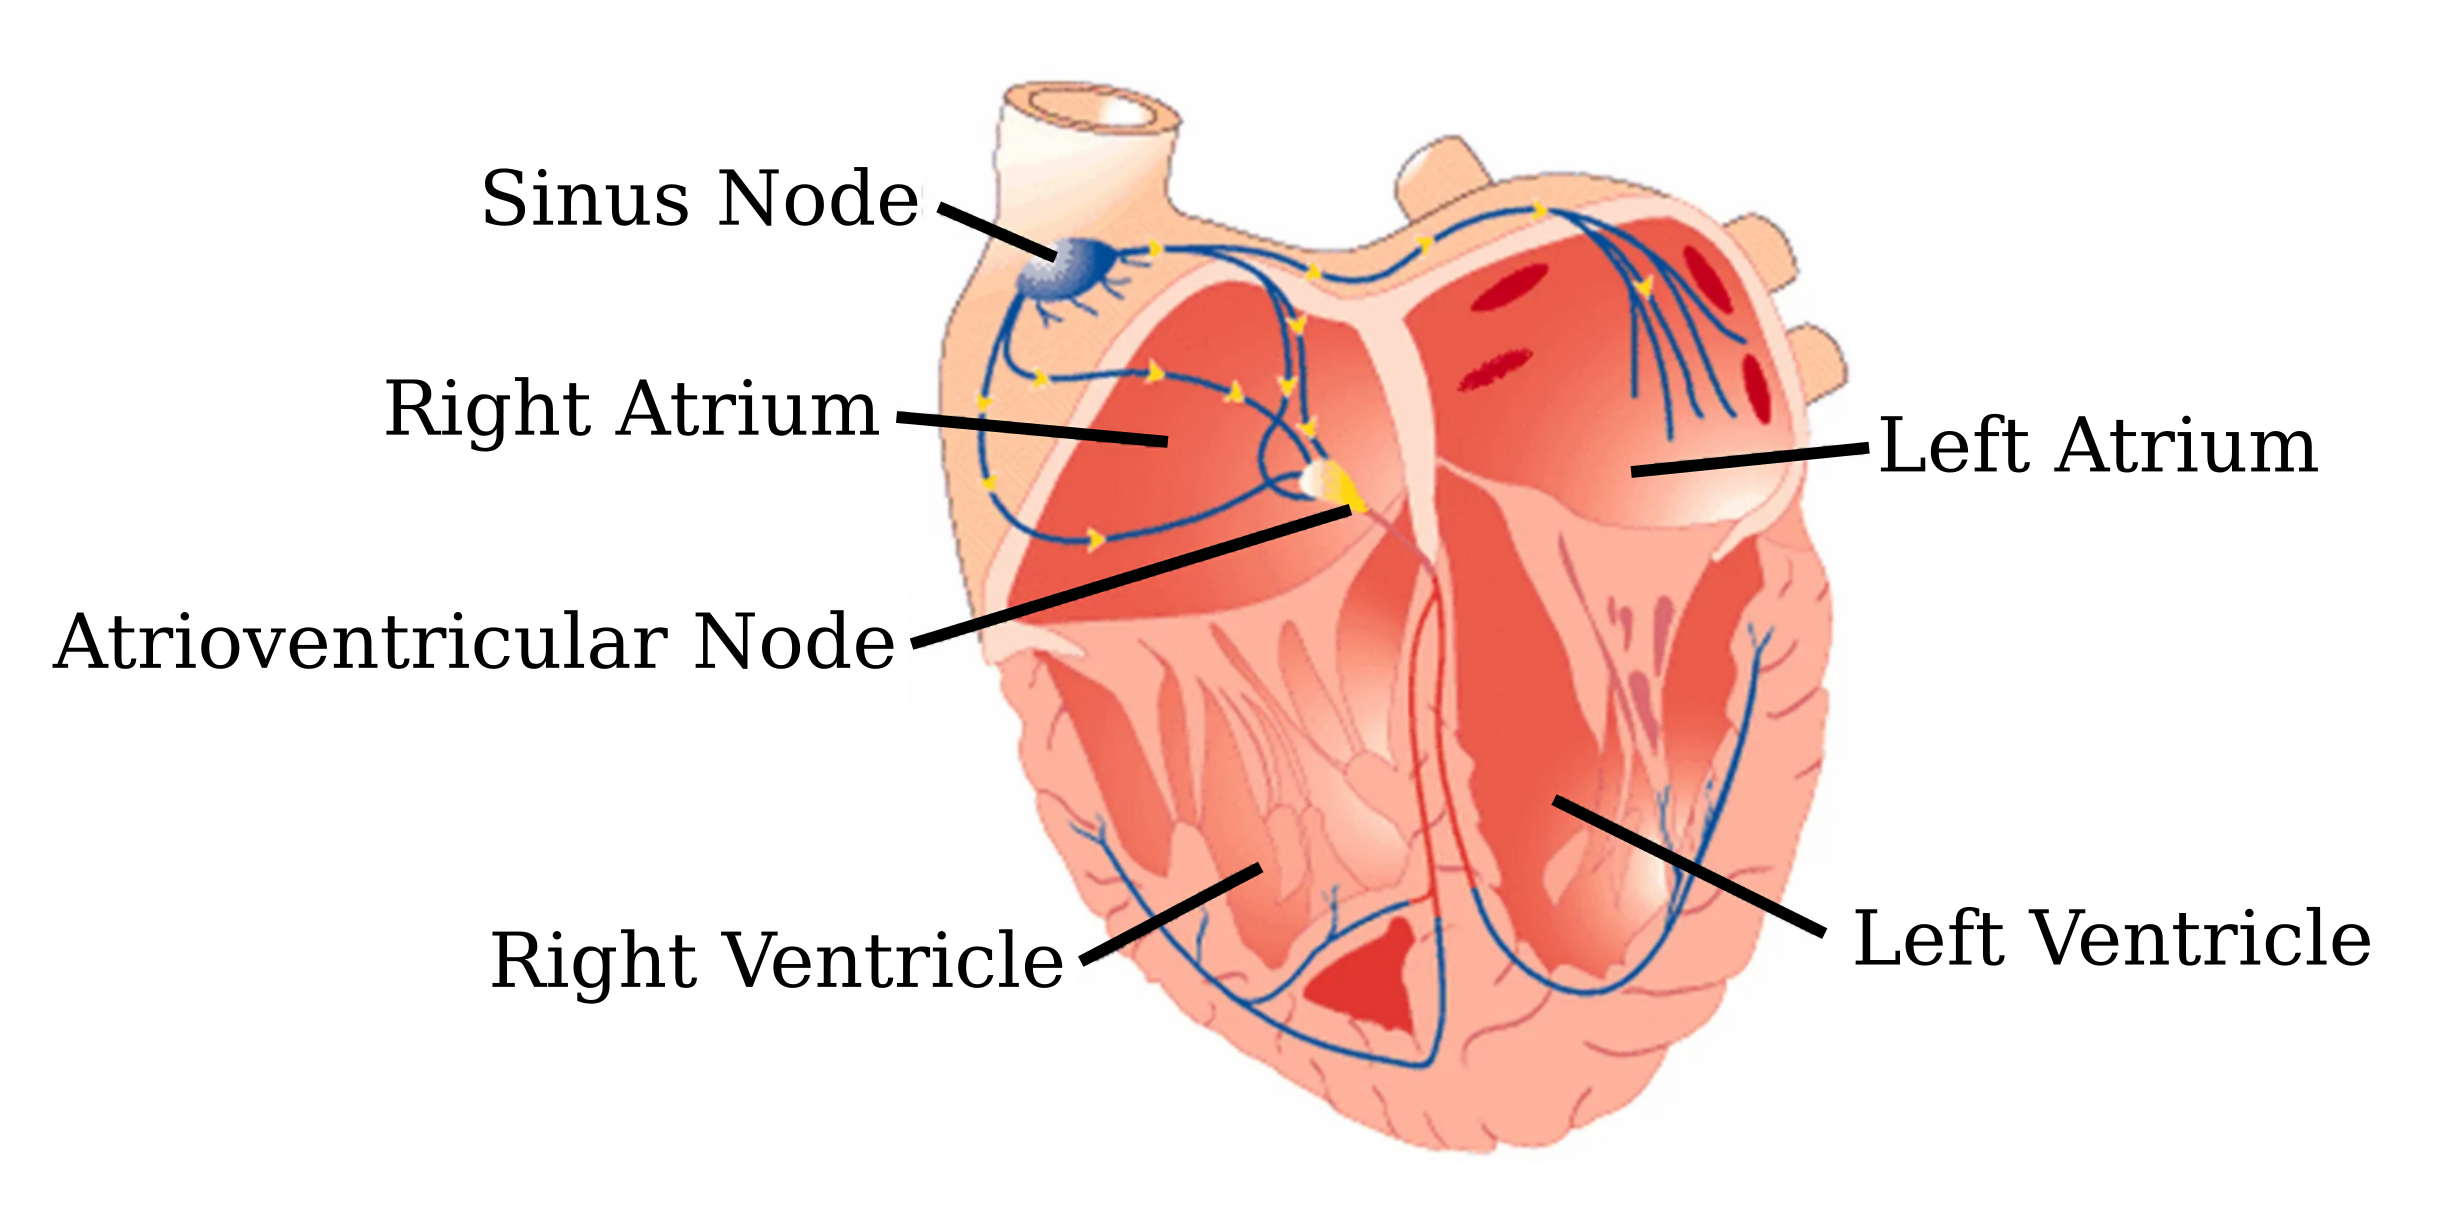
\includegraphics[width=1.0\textwidth]{figures/heart_physiology.png}
	\caption{Physiology of the heart. Copyright 2019 by a-fib.com}
	\label{fig:heart_anatomy}
\end{figure}

\subsection{Cardiomyocytes}
Understanding cardiomyocytes as smallest functional unit of the heart muscle is the key to understand the heart global behavior. An electro-chemical signal propagates through gap junctions between cardiomyocytes and let them contract individually but coordinated, that the heart shows a pump effect.
In figure (\ref{fig:cardiac_excitation}) the temporal progression of three interdependent processes are sketchily shown. The blue curve shows the action potential, a temporary characteristic deviation of the membrane potential of a cell, from the rest potential. The potential is dependent on the ion-concentration within the cell. The red line shows the Calcium transient which is indirectly responsible that the cell contracts, by activating myofilaments (proteins). The Calcium-ion channel is only one kind of multiple channels to control the potential in terms of polarization, hyperpolarization or depolarization \cite{mycardium_lecture}.
The dotted green line shows the intensity of contraction, which is a delayed reaction of the action potential course. Their temporal dependent behavior is called excitation-contraction coupling (ECC).  On the other hand it is signaling receptors\footnote{DHPR-receptor (Dihydropyridine receptor), it is a Calcium-dependent channel and functions as a voltage sensors, for further information see \cite{woodcock_cardiomyocytes_2005}.} to prevent the cell from further Calcium-ions (Ca$^{2+}$) to get into the cell. With exchanging Calcium-ions, the cardiomyocytes 'communicate' with each other, and allow the actions potential to be transferred that they act as an electrical neighbors-wise coupled system and are able to contract coordinated.
The action potential has a refractory period where it does not show any response to a stimulus from another cell, which lasts around 250 milliseconds, to protect the heart. This period is relatively long in comparison a nerve cell, which has a refractory period of around 2 milliseconds. 

\begin{figure}[ht]
    \center
    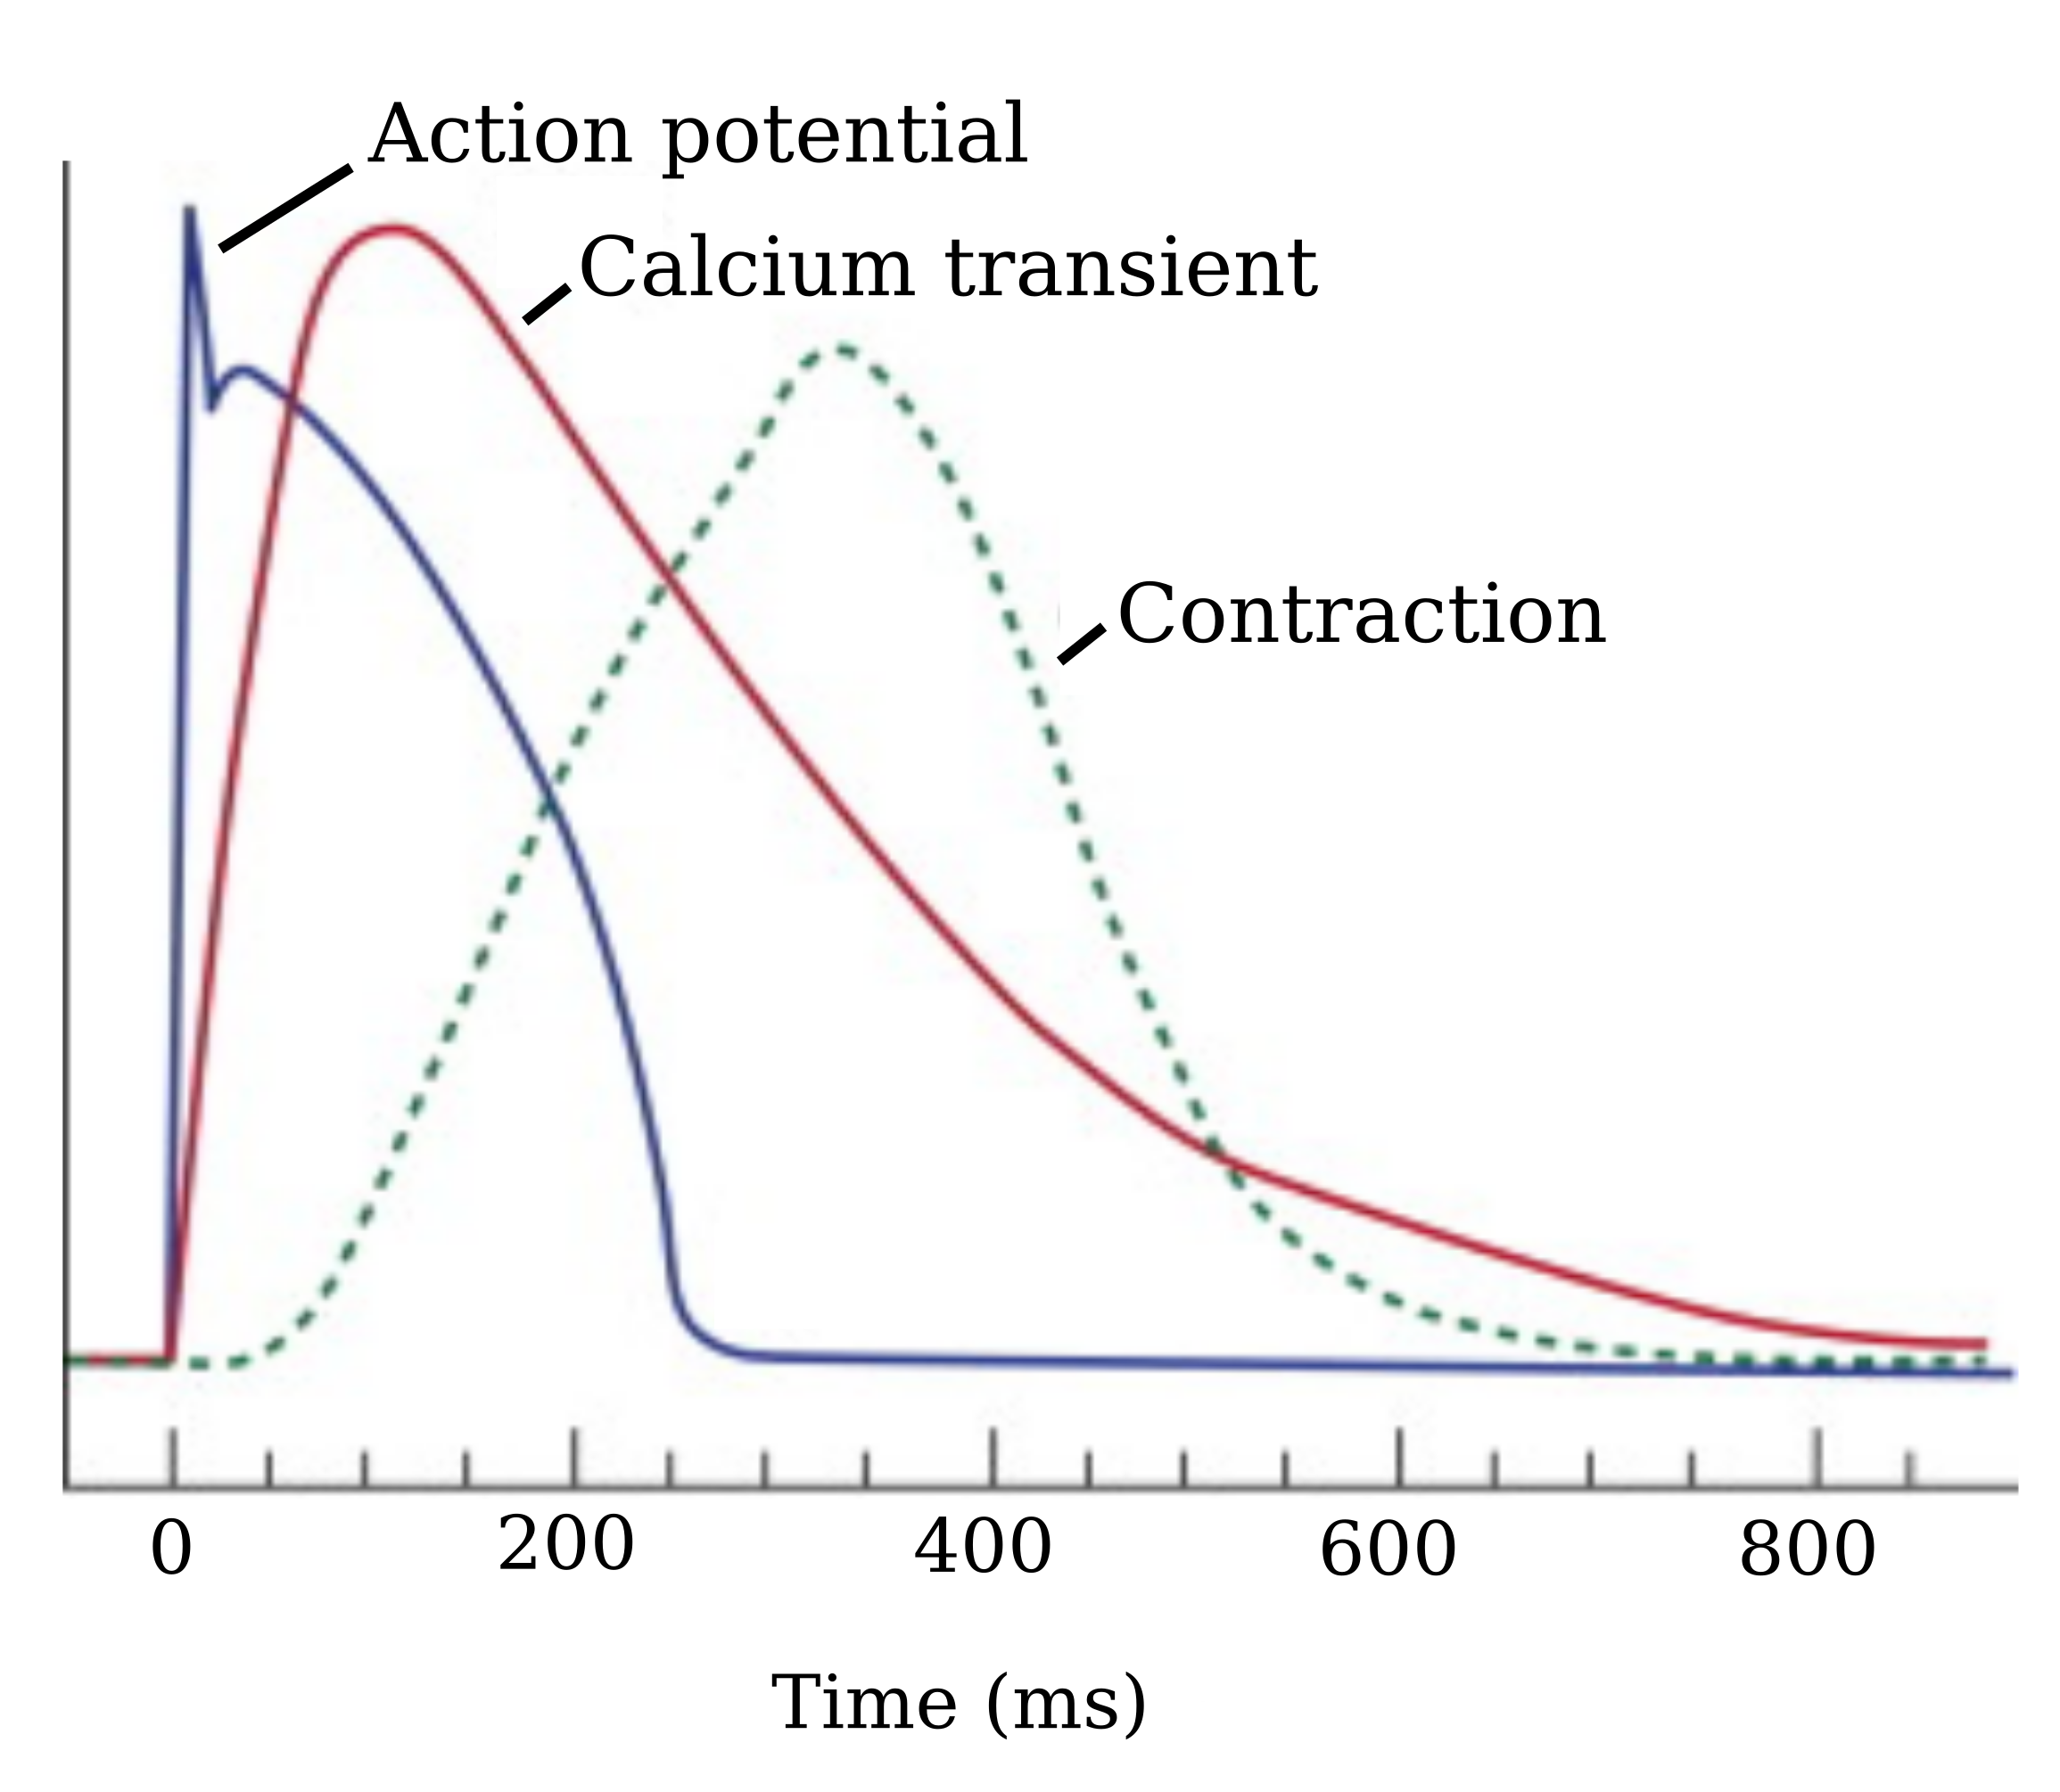
\includegraphics[width=0.7\textwidth]{figures/caradio_excitation.png}
	\caption{Physiology of the heart. Copyright 2020 by sciencedirect.com}
	\label{fig:cardiac_excitation}
\end{figure}

%\subsubsection{Activity of the heart, Arrhythmias}

%Normal sinus rhythm, spiral waves, or just chaos?

%\subsection{Models of the heart-activity}
%\textbf{The FitzHugh–Nagumo model}\\

%\begin{align}
%    \dot{v}=v-\frac{v^3}{3}-w+I_{\text{ext}}\\
%    \tau\dot{w}=v+a-bw.
%\end{align}

%The parameter $I_{\text{ext}}$ is the expression for an external stimulus. The FHN Model is a relaxation oscillator\\

%\textbf{The Barkley model}\\
%\begin{align}
%    \dot{v}=v-\frac{v^3}{3}-w+I_{\text{ext}}\\
%    \tau\dot{w}=v+a-bw.
%\end{align}
%\input{content/theory/ecg}

\section{Electrocardiography}
In broad terms, the electrocardiography can be understood as a spatial summation of the potential (blue line in figure (\ref{fig:cardiac_excitation})) of all individual cardiomyocytes after a diffusion process. Therefore, it can be regarded as the determination of the electro-chemical behavior of the heart\footnote{We will ignore possible noise from other organs like the brains which is electro-chemical active as well, nevertheless the heart dominates the ECG-signal}. The potential is measured by electrodes (non-invasive on the torso or minimal-invasive).
A widely known setting is the 12-lead-ECG, where 9 electrodes are used to form 12 leads whose potential is determined individual subtraction from other electrodes or virtual electrodes\footnote{See chapter (\ref{cap:potential_reconstruction}).}. In the following I will explain how the potential can be reconstructed in detail.
%While the forward problem, the propagation of potentials through the body, can be simulated unambiguously as a diffusion process, the inverse direction is mathematically ill-posed. 
\subsection{Potential Reconstruction}\label{cap:potential_reconstruction}
For an ECG it is necessary to have at least two electrodes which form a lead, by subtracting one signal from the other as a reference. The resulting 'normalized' signal is the spatial potential difference between them. It is also possible to form 'virtual' electrodes by taking the average of multiple electrodes. A standard lead-system is the already mentioned 12-lead ECG, its signal is based on a defined electrode positioning as shown in figure (\ref{fig:12-lead-ecg}).

\begin{figure}[ht]
    \center
    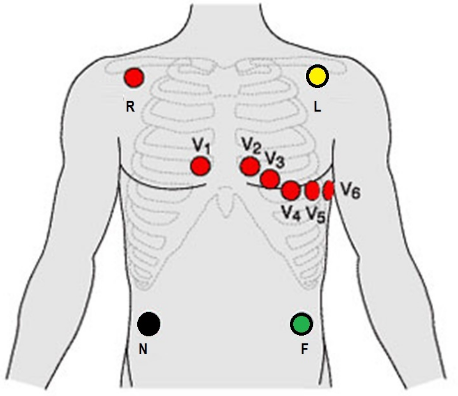
\includegraphics[width=0.7\textwidth]{figures/ecg_12_lead.png}
	\caption{12-lead ECG, positioning. Copyright 2020 by firstaidforfree.com}
	\label{fig:12-lead-ecg}
\end{figure}
By subtracting the measurement of an electrode with another reference- or virtual electrode, one can gain information about the spatial potential gradient along the vector between these electrodes. The signal of each electrode of $V$ calculates its potential by subtracting with the virtual electrode, defined by the average of $R$, $L$ and $F$ \cite{12lead_ecg}.

\subsection{History}
While the 12-lead ECG is a widely used technique on modern medicine, in the history of ECG, Einthoven was able to identify various cardiac arrhythmias with a setup, based on three electrodes, which is known as Einthoven's triangle\cite{conover_understanding_2003} (see figure (\ref{fig:einthoven_triangle}).
This setting improved the first ECG for human in 1887 by Augustus D. Waller \cite{waller_1887} in terms of robustness and sensitivity. Electrodes are attached on the left and right arm, and on the left leg, which are forming three leads (staying in the terminology of 12-lead ECG, one might call it 3-lead ECG). However, this approach is no longer relevant for modern medical information gathering.

\begin{figure}[ht]
    \center
    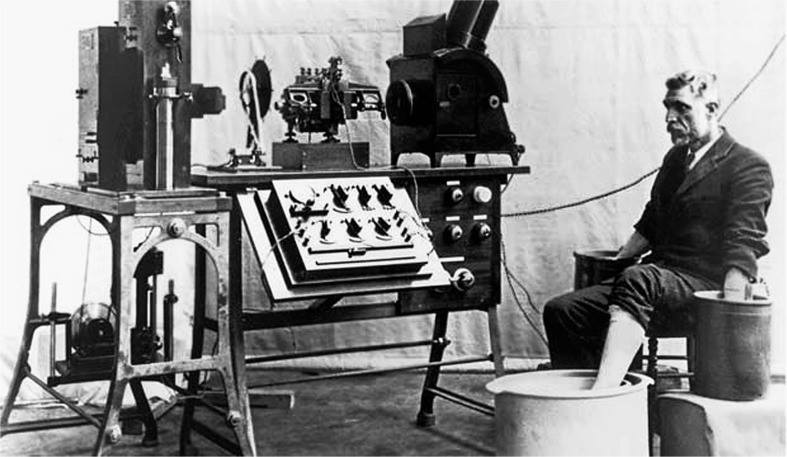
\includegraphics[width=0.7\textwidth]{figures/einthovens_triangle.png}
	\caption{Einthovens Triangle, three electrodes (left- right hand and feet) form a triangle and three leads.}
	\label{fig:einthoven_triangle}
\end{figure}


\section{Signal Propagation from the Heart}
\textbf{The forward problem}\\
The phrase forward in a dynamic system is based on the idea, that one have a known structure which emits a propagating signal 'forward' through a system. The inverse problem is therefore the tracing back of an emitted signal to obtain information about the mentioned structure and its properties.
To define a forward formulation and its relation to the inverse case, firstly we assume that the problem is linear. Existing approaches which don't consider movements of the heart through beating or breathing of a patient, are able to assume a forward propagation in a mathematical linear manner\cite[p. 241f]{sundnes_computing_2006}. The propagation can thus be written as 

\begin{align}
    \label{eq:linearity}
    \varPhi_{\text{ecg}} =\textbf{A}\cdot\varPhi_{\text{heart}}.
\end{align}

In this notation, $\varPhi_{\text{heart}}$ is the epicardial potential and $\varPhi_{\text{ecg}}$ the potential measurements of the ECG-electrodes. Both are expressed in form of a vector. Because of the linearity the forward operator $\textbf{A}$ is a matrix.\\

\textbf{Limitations of the linear formulation}\\
For simplicity we assume that there is no additional or non-linear noise, it would increase the complexity of the model and the search for $\textbf{A}$ would become even very impractical. It is not possible to include geometric noise which lead from the contraction of the heart muscles only with additional terms in a static formulation of the problem, because the contraction correlates with the excitation of cardiomyocytes with a temporal delay.
By considering the fact that there is a temporal delay between measurable excitation through the ECG-electrodes and the contraction of the muscle, one might argue that the noise from this source is not significant when the problem is not including time embedded coordinates (the temporal behavior). However, the problem arises that when time is integrated into the coordinates\footnote{Time-embedding in a linear manner is possible with delay coordinates} and the geometric noise might becomes significant noticeable.
Furthermore, in clinical measurements the movement of the torso coming from breathing, which is subject to a certain amount of random behavior, could lead to a significant noise. 
On the one hand it is possible to include the time in the linear formulation through delay coordinates, on the other hand the time-dependent geometric noise becomes increasingly relevant. Therefore, the entries of the forward-matrix with included delay-coordinates $\textbf{A}$ are not exact, also because of difficulties to define the geometry satisfying\footnote{The individual geometry of a patient's torso and its heart can be provided by for example Magnetic Resonance Imaging (MRI) or Computed Tomography (CT).}. These limitations have be considered by the assumption of a linear signal propagation for the forward problem, and the difficulty to find a good assumption for the operator might lead to practical problems. Every inverse-ECG formulation based on ($\ref{eq:linearity}$) has to face these problems, and in general the inverse mapping requires regularization methods to improve the robustness of the solution against the mentioned noise.
Regarding a biological reasonable solution as best solution of the model is also an important aspect of regularization. At the same time, with excluding possible solution it is possible that there is a loss in generalization. The solution of the problem ($\ref{eq:linearity}$) can be formulated in the question: What is the best prediction for $\varPhi_{\text{heart}}$ that the resulting ECG-signal after applying the operator $\textbf{A}$ on $\varPhi_{\text{heart}}$ is the as close as possible to the true ECG-distribution. 

%The formulation implies that the operator has to be known for the solution. In the following chapter I will introduce a $\mathcal{L}_2$-regularization method also known as Tikhonov regularization or in general Ridge-regression.
%and why the operator has to be known for this technique.

%Otherwise it might not be ignorable isn't the case if the time is embedded in the describtion of the data.

%(in clinical measurements) the movement of the torso coming from breathing. On the one hand it is possible to include the time in the formulation an therefore the temporal behavior of the dynamic and signal propagation with keeping the linearity, but on the other hand the geometric noise

%is the dominating source for the potential measurements $\varPhi_{\text{ecg}}$ of electrodes.

%$\textbf{b}$ is regarded as noise and being a vector, as well as $\varPhi_{\text{ECG}}$, holded to be the measurement (in this context ECG-signals).

\section{The inverse Problem}
In classical approaches to solve the inverse problem of ECG\footnote{Like Tikhonov regularization or Truncated SVD (TSVD)\cite{macfarlane_comprehensive_2010_page_309}.}, the forward formulation is determined first, which regularized inversion leads to a possible inverse solution. This means that the problems of the forward operator/mapping as already described, are also relevant for the inverse solution. In addition, by assuming a linear propagation, the inverse solution of (\ref{eq:linearity}) is not unique, which lead to ill-posedness.
Before giving an mathematical definition for the inverse formulation, the phrases \textit{well-posed} and \textit{ill-posed} will be introduced.  \textit{Ill-posedness} is regarded as a property from which follows that a solution cannot be given exactly. 
In the following I will show why this inverse problem is ill-posed and several state-of-the-art methods how to handle this property with regularization.

Following the definition of Jacques Hadamard \cite{hadamard_1902} a problem is well-posed if

\begin{enumerate} 
    \item A solution exists.
    \item The solution is unique.
    \item The solution depends continuously on the data.
\end{enumerate}

A problem is \textit{ill-posed} if it fails to satisfy one or multiple of these conditions, in other words if it is not \textit{well-posed}.\\
Even if the linearity is given, the inverse problem of ECG is still ill-posed, which means that there is no closed function of the form $\varPhi_{\text{heart}}\equiv f(\textbf{A},\textbf{b},\varPhi_{\text{ecg}})$ which maps the ECG-signal on the exact epicardial potential distribution (different potential distributions can lead to the same ECG-signal). It is not necessarily given that the matrix is squared and regular, which is the reason why there is not reliably a solution given by the assumption that the matrix is invertible. While the problem is not solvable in an exact way, the task leads to the search of the most probable source of the ECG-potential. To give a biologically realistic prediction of the inverse problem despite this property, there are various regularization methods which will be introduced in the following chapter.\\


\section{Common Regularization Techniques, State of the Art and Limitations}
The ultimate goal for the inverse problem of ECG would be to map the whole epicardical potential distribution based on the electrocardiogram, it is clear that this goal is utopian, but biological models can already produce relative accurate results. 
In the following, I will discuss two models that represent a regularization of the linear model. Nevertheless, these methods do not offer solutions based on biological knowledge, but only rely on empirical measurements.

The approaches for non-invasive inverse potential mapping through electrocardiography can be defined after Matthijs Cluitmans et al. \cite{cluitmans_noninvasive_2015} from 4 assumptions they make or models they use:

\begin{enumerate}
    \item The cardiac source.
    \item The signal propagation through the body.
    \item The model output, being the body-surface potential via ECG.
    \item Regularization methods to overcome the mentioned problems in the inverse mapping
\end{enumerate}
This classification of approaches includes the assumption that a forward-model is necessary to solve the problem.
However, once the patient-specific forward-matrix is estimated (firstly we focus on the linear assumption of point 2.), which maps the potential distribution from the cardiac source to the body-surface potential, the formulation of the inversion of the matrix $\textbf{A}$ can be performed. In the following I will only consider a potential-based formulation\footnote{with the wave-front-formulation they are the most often used cardiac source representations\cite{cluitmans_noninvasive_2015}.} of the cardiac source, as it is the formulation-model for the following approaches in this work. Solutions, consisting of the pseudoinverse\footnote{The inverse (not pseudo) $\textbf{A}^{-1}$ is not necessarily defined.}
$(\textbf{A}^{\text{T}}\textbf{A})^{-1}\textbf{A}^{\text{T}}$ are extremely sensitive to noise and may not be able to make biologically realistic predictions for the epicardial potential distribution. In general the problem can be redefined as the minimum of the euclidean distance between the prediction of a model $\mathcal{F}$ and the true potential distribution 

\begin{align}
    \label{eq:linear_regression}
    \min&\parallel\textbf{A}\mathcal{F}\varPhi_{\text{ecg}}-\varPhi_{\text{ecg}}\parallel_2^2
\end{align}

where $\mathcal{F}\varPhi_{\text{ecg}}$ can be regarded as a fit to the data with $\mathcal{F}\equiv(\textbf{A}^{\text{T}}\textbf{A})^{-1}\textbf{A}^{\text{T}}$ as closed form for the best solution. In other words, $\mathcal{F}\varPhi_{\text{ecg}}$ is the best solution, that the forward operator would map $\mathcal{F}\varPhi_{ecg}$ as close as possible to the corresponding true $\varPhi_{ecg}$. This formulation is well-posed with the given solution model for $\mathcal{F}$, nevertheless this does not mean that the solution is biologically realistic.
A common response to this problem is regularization, giving additional information about the biological nature are a technique to adapt the inverse problem to give a more realistic solutions. It furthermore might lead to a more robust solution against noise. 
In the following I will go through a few regularisation methods.

%While the assumptions of the forward propagation are not always linear, I will use it and its regularization methods as comparison for the machine learning approach, because it is the most known assumption.
%On the other hand I will introduce a few machine learning approaches which are used to solve special posed problems of the inverse ECG like the classification of diseases. Broadly the state-of-the-art machine learning approaches doesn't consider cell-level inverse-mapping and concentrate more on the classification problem. 
%[Zittieren: Arrythmia classification, ECG-classification in general, myocardial infarction...]: Mostly detection and classification but no potential mapping.
%While the most model consider a linear forward propagation (1) as model, \\

%\textbf{Tikhonov Regularization}\\
As a standard regularization method the \textbf{Tikhonov Regularization}\cite[p. 126]{willoughby_solutions_1979} solves the problem (\ref{eq:linear_regression}), with a modified linear regression model by constraining the magnitude of $\varPhi_{\text{heart}}$ with adding a penalty term. The problem is differently formulated as 
\begin{align}
    \label{eq:linear_regression_tikhonov}
    \min&\parallel\textbf{A}\mathcal{F}\varPhi_{\text{ecg}}-\varPhi_{\text{ecg}}\parallel_2^2+\lambda\parallel\mathcal{F}\varPhi_{\text{ecg}}\parallel_2
    %\label{eq:linear_regression_tikhonov2}
    %\min&\parallel\mathcal{F}\varPhi_{\text{ecg}}-\varPhi_{\text{heart}}\parallel_2^2+
    %{\underbrace{\lambda\parallel\mathcal{F}\varPhi_{\text{ecg}}\parallel_2}_{\substack{\text{Tikhonov}}}}
\end{align}

\cite{ito_inverse_2015}. 
The term (\ref{eq:linear_regression_tikhonov}) gives a closed form for the best prediction as
\begin{align}
    \label{eq:closed_tikhonov}
    \mathcal{F}=(\textbf{A}^T\textbf{A}+\lambda\textbf{B})^{-1}\textbf{A}^T,
\end{align}
where $\textbf{B}$ becomes the identity-matrix in case of the zero-order Tikhonov regularization. Fluctuation in a high frequency, with other words on a small scale are possibly not visible on the ECG-signal due the property of a diffusion process of showing the behavior of a low-pass-filter. In other words the term for (\ref{eq:closed_tikhonov}) with $\lambda=0$ (no regularization) could lead to a solution with biological unreasonable fluctuations. Therefore, $\lambda$ has to be adjusted to ensure a better result.
More advanced methods are taking into account the temporal behavior, that the constrained solutions which are temporally close to each other, should be reasonable close in their epicardial potential distribution as well \cite{oster_use_1992}\cite{time_space_1995}. Another approach from Brooks et al. \cite{brooks_augmented_1993} augments the Tikhonov regularization and considers multiple constraints with an additional term to ensure the temporal smoothness of the solution. 

No matter how good the regularizations are, the quality of a solution is estimated by the difference between the true ECG signals and the 'practically perfect' forward calculation of this solution. Of course, the forward operator is not perfect as already discussed. Furthermore, the solution are rather of mathematical nature, and less physiologically directly justifiable and the regularizations rely on a static geometry of the unique heart and torso.

For practice for clinical applications, one could ask does it worth it the torso and heart-mapping with CT or MRI to generate a patient-unique inverse ECG. 

Finding an extended inversion model which is reliable on different types of bodies, heart shapes and slightly varying ECG-positions, may be advantageous due to possible economic or practical difficulties. We note that regularization, based on the assumption in (\ref{eq:linearity}), need the patient-specific geometric model of the whole heart and torso as well as the forward operator to find a solution for the inverse problem. 
To hide this requirement of a model, aim of this work is to find an approach which is able to 'learn' the inverse solution without any knowledge about the forward operator, just by giving the epicardial potentials and ECG-signals. 
Can we on the other hand ask a more specific question about what is going on at the heart. This could be the localization of the source of a spiral wave, which could initiate a more targeted ablation. Limits of a model with usage of methods of machine learning, which are increasingly used to find pattern in unknown data, is aim of this work.

%\input{content/methods/neural_architecture}

\section{Methods}
\subsection{Simulation of ECG-Signals}\label{cap:simulation}
The analysis of ECG signals is based on the simulation of a pig heart, the 3D structure is from a computed tomography scan (CT-scan).
To generate ECG signals, the model for the activity in terms of extracellular potential of the heart is based on a pseudo-bidomain model. Especially when simulating an ECG the bidomain formulation is considered to be the most detailed biophysical approach \cite{bishop_bidomain_2011} but computational cost intense. To reduce the cost, the model includes the assumption, the intra- and extracellular domains to be anisotropic, but to the same degree. The bidomain model is then simplified to the mentioned pseudo-bidomain model, so that for the extracellular potential the equation 
\begin{align}
    C_m\frac{\partial V_m}{\partial t}+I_{\text{ion}}=\nabla(\sigma_m\nabla V_m)
\end{align}
applies, where $C_m$ is the membrane capacitance per unit area, and $I_\text{ion}$ is the ionic current density through the membrane. The parameter $\sigma_m$ can be regarded as bulk conductivity\footnote{For further derivation and explanation see \cite{bishop_bidomain_2011}.}.

The local ion flux is simulated with the FitzHugh-Nagumo model \cite{fitzhugh_1955}.

The 3D model of the pig-heart consists of around 32000 connective points to define a finite element mesh. The differential equations are solved with help from the open-source framework DOLFIN \cite{LoggWells2010a} in Python, the FitzHugh-Nagumo equations are solved the implementation of the Runde-Kutta solver from scipy \cite{2020SciPy_NMeth}.

The main simulation framework is provided by Baltasar Rüchardt \cite{baltasar} and contains four steps:\\
\begin{itemize}
    \item augmented monodomain simulation,
    \item reconstruction of the extracellular potential in the heart,
    \item diffusion process in the bath,
    \item reconstruction of the ECG.
\end{itemize}

The potential propagates as a diffusion process through the bath, it can be regarded as a process which blurs the propagating potential. In the last step, because each electrode contains multiple points, the signal is integrated over each of these subsets. Figure (\ref{fig:pig_heart_in_bath}) shows the simulation setup with the heart inside the bath with the included ECG-electrodes, attached on the two panels from two sides.

\begin{figure}[ht]
    \center
    \hspace*{-2.45cm} 
    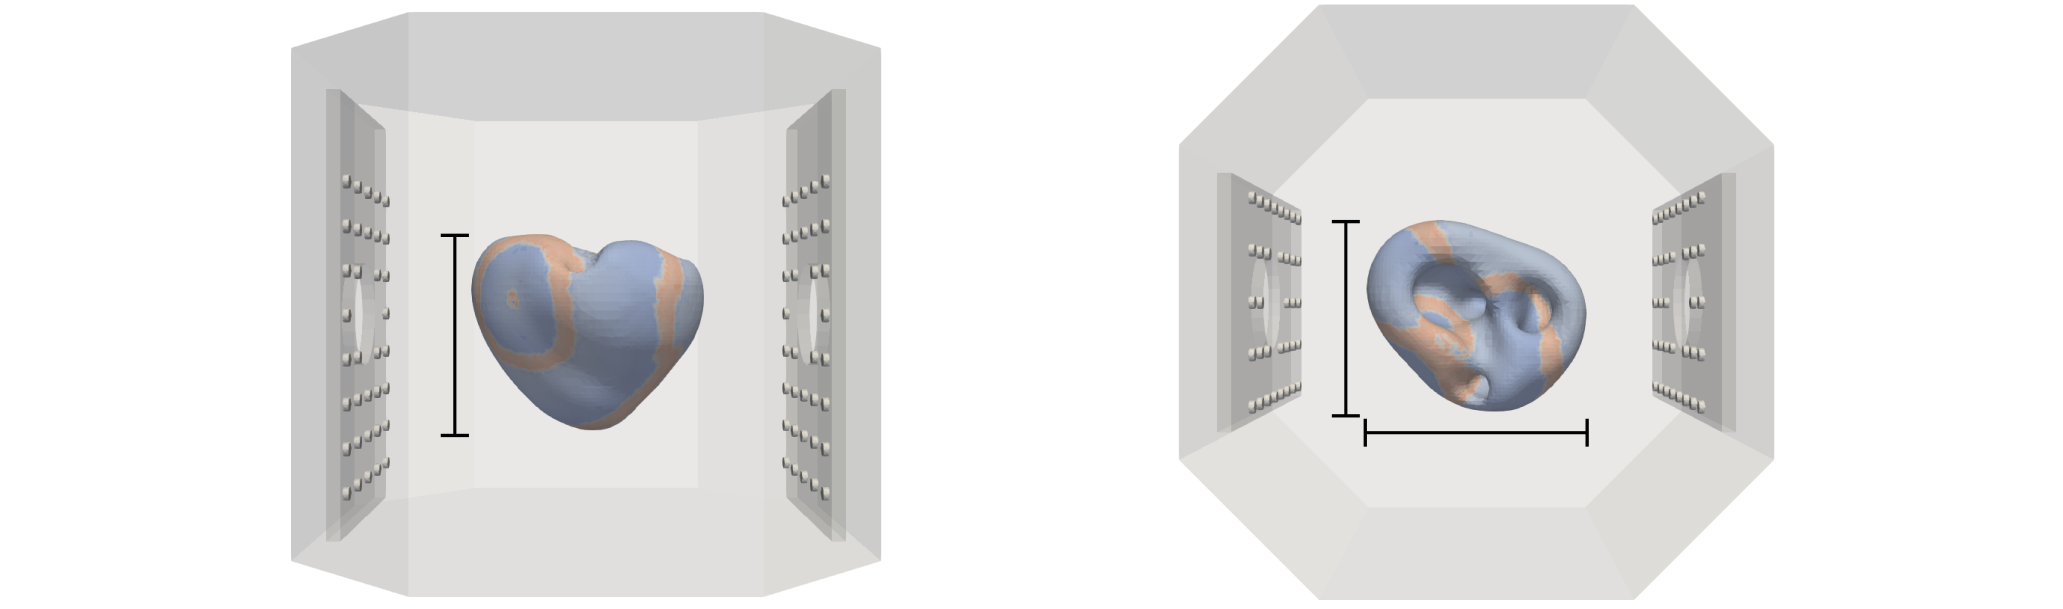
\includegraphics[width=1.4\textwidth]{figures/simulation_setup.png}
	\caption{Simulation of a pig heart, visualized with paraview \cite{paraview}, the panel on the left and right side on each image contain 64 electrodes for the simulated electrocardiography, as they are placed in the experiment in \ref{cap:concentricwave}.}
	\label{fig:pig_heart_in_bath}
\end{figure}



\subsection{Convolutional Neural Network for Concentric Wave Localization}
\label{convnet}
ECG-signals are a time series with including multiple channels. While the analysis of a time series, includes a variety on different fields like stock-market prediction, weather prediction, traffic-prediction, denoising of signals or speech analysis, a broadly used technique through these problems involves convolutional neural networks (CNN), which is also the base for the model in this work to analyse the ECG-signals. 
As visualized in (\ref{fig:cnn_architecture}) the CNN consists of seven convolutional blocks consisting of a

\begin{itemize}
    \item Convolutional layer,
    \item Batch-Normalization layer,
    \item Activation-function,
    \item Dropout layer.
\end{itemize}
Having an input of 256 time steps at 64 channels, each convolutional block is shrinking the dimension through a stride of two, by the factor of $\frac{1}{2}$, that the time-series from the input is represented after the seven convolutional block by a row of four neurons with 256 channel\footnote{The number of channel is a hyperparameter of a convolutional layer, for the exact setting, see \ref{cap:neuralnetworkarchitecture}.}. A fully connected layer follows, on which attached is a batch-normalization layer and ReLU-function, and an additional linear layer with a linear-activation function.\\

\begin{figure}[ht]
    \center
    \includegraphics[width=0.7\textwidth]{figures/neural_architecture.png}
	\caption{Basic Neural Network Architecture}
	\label{fig:cnn_architecture}
\end{figure}


\section{Experiments}
%\section{Localization of Excitation Sites from Simulated ECG}
With potential measurements from a multichannel-ECG it is impossible to estimate the exact activity of a single myocyte due to its ill-posedness. 
Nevertheless, the global activity of a heart can be influenced by single cells due to the low-resistance coupling of neighbouring cells and the resulting signal propagation. Because of this significant influence of local activity we want to explore the limits of a model, which predicts spatial information where a single heart muscle cell or a collective of cells show certain dynamic properties that significantly determine the global activity of the heart. This can be done for example by stimulating a certain small area in a periodic pattern, with the adjustment that the periodicity and strength of the pulse dominates the global activity.

In previous chapters, an attempt was introduced, which includes delay coordinates to the input of a model to solve the inverse problem. This strategy does make it possible to have an encoded information about the temporal behavior, nevertheless the spatial information, with other words the geometry of the heart is not taken into account\footnote{One have to mention that the geometry is expressed with the linear operator $\textbf{A}$, therefore the spatio-temporal behavior is indirect considered in the data set and its prediction for $\varPhi_{ECG}$}. A strategy to include this into the model, is to run a variety of ECG measurements based on the signal of the same heart respectively hearts-geometry with as different dynamics as possible. As consequence the ECG-signal contains in an encoded way the behavior of different dynamics on the same heart. 

We start with a very simple experiment to have an idea about the limits of this strategy. In the following I will introduce an experiment which realizes the mentioned steps.

\subsection{Concentric Wave Localization}\label{cap:concentricwave}
In 1024 simulations\footnote{The simulation setup and technique is explained in \ref{cap:simulation}.}, concentric waves are generated in a periodic pattern from a random point on the hearts surface, which then spread over the entire heart. The activity in each simulation is therefore significantly influenced by only one source. No sinus rhythm or a spiral wave have yet been simulated, as is the case in later experiments\footnote{These experiments are planned, see in the chapter outlook.}, that interactions between 'disturbances' and another activity can be excluded. The ECG signals thus 'see' the behavior of a continuous wave over the heart's geometry, which has a different origin in each simulation.

The goal in the first approach is to predict the source of a concentric wave, which is produced by an external stimulus $I_{\text{ext}}$ at a random chosen subset of the heart $\Omega$. The spread of this area is so small that it contains only a few elements. The signal propagates as a concentric wave through the whole heart. The external stimulus in the simulation is a function $I_{\text{ext}}(t, \textbf{s})$ which is periodic at certain area $\Omega$. It is defined as 

\begin{align}
    I_{\text{ext}}(t, \textbf{s})=
    \begin{cases}
        I_0\cdot\text{Rect}(t) & \mbox{if } \textbf{s}\in\Omega \\
        0 & \mbox{else}\\
    \end{cases},
\end{align}
with
\begin{align}
    \text{Rect}(t):=
    \begin{cases}
        1 & \mbox{if } t\text{ mod }P < d \\
        0 & \mbox{else}\\
    \end{cases},
\end{align}
where $P$ is the duration of a period and $d$ the length of the stimulus. The strength of the stimulus is given by $I_0$.\\

Therefore, the simulation setup is the same in every simulation, only the source of the concentric wave is varied. Figuratively spoken the adjustable weights $\textbf{W}$ of the neural network $\mathcal{F}_{\textbf{W}}$ which learns to identify the source of the concentric wave, learns to give an encoded expression of the globally constant settings like the geometry of the heart and the position of the electrodes or the differential equations for the spatio-temporal activity through its weights.

\subsubsection{Data Preprocessing}
Each simulation gives an output with 70 time series of length 1600 time-steps from the channels in the configuration (I) from (\ref{cap:simulation}). The first 600 time-steps are regarded as initialization-period and therefore not considered in the training process, which ensured that the concentric wave generation already shows globally influence. The potential is reconstructed by subtracting each time-series with the signal from a virtual electrodes which can be regarded as being in the center of the heart. This ensures that the spatial potential gradient is calculated in as many directions as possible. The virtual electrodes is built by the average of the four reference electrodes, visualized in figure (\ref{fig:simulation_concentric_wave_overview}).
In the next step, 80\% of the data will be used for training, the remaining 20\% for validation to ensure the generalizability of the model on unknown concentric waves sources.

\begin{figure}[ht]
    \centering
    \hspace*{-1.7cm}
    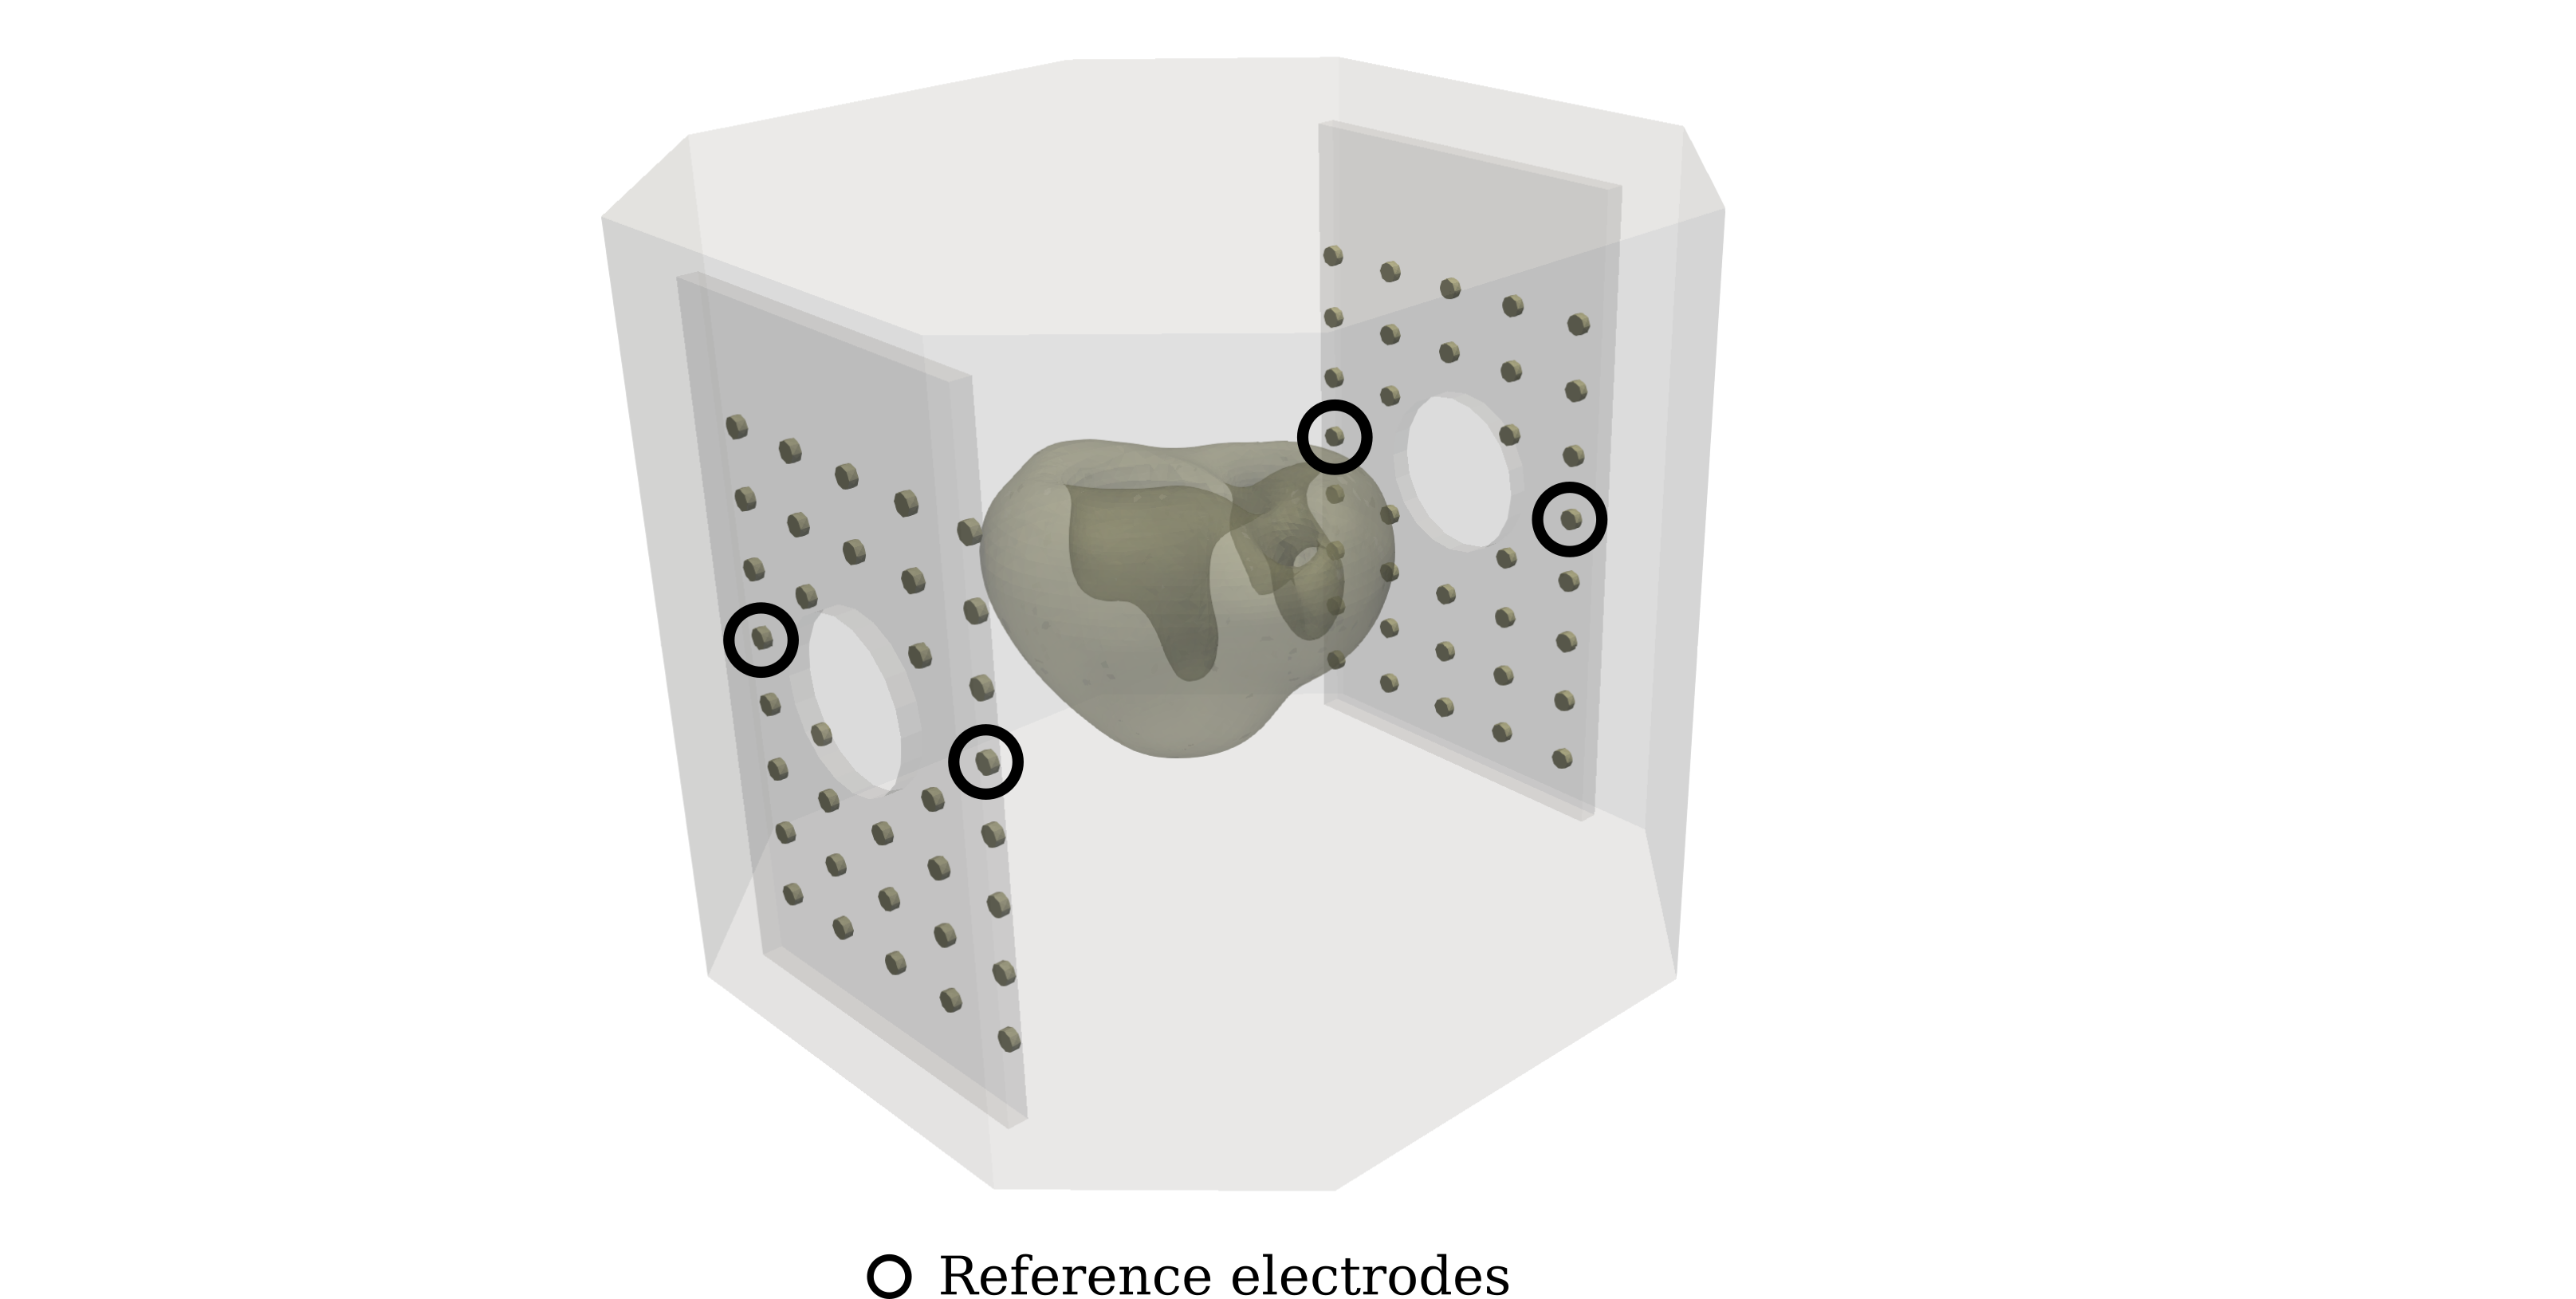
\includegraphics[width=1.4\textwidth]{figures/heart_overview_inkscape.png}
	\caption{Simulation setup with the reference electrodes (marked with black circles).}
	\label{fig:simulation_concentric_wave_overview}
\end{figure}

From the remaining 1000 time-steps on each simulation in the training- and test-set, 8 sub-sequences of length 256 are picked at random times. The simulations have an average period length of 223 time-steps, therefore the length of a single sub-sequence includes around 1.15 period-length. 

For 1024 simulation the amount of sub-sequences result into $1024\cdot8=8192$ where 6536 of them are used for training, and 1640 for testing\footnote{Because of technical problems, two simulation have been excluded, therefore 16 sub-sequences are missing.}. The choice of random starting-points comes from the idea, that the model should be invariant through time-shift in its prediction. With this property the model is able to give nearly the same prediction on different phases, without being dependent on a certain selection.\\


\subsubsection{Training-Process}
The training/optimization process is based on the adjustment of the model immanent weights. For this purpose the stochastic gradient descent method Adam (c.f. section \ref{cap:optimizer}) is used. The method does an update-step with including a batch of size 256, including random chosen samples. The hyperparameters of the optimizer are as in the tensorflow-API \texttt{keras} by default as $\alpha=0.001$ (learning-rate), $\beta_1=0.9$ $\beta_2=0.999$ and $\varepsilon=1\cdot 10^{-7}$.
During the training, after the loss did not decrease for 32 epochs (plateau-phase), the learning-rate will be decreased by a factor of 0.8. If this phase lasts longer than 256 epochs, the training will be stopped.

\section{Results}
In the following I present the performance of the convolutional neural network (c.f. section \ref{convnet}) which is trained to predict the source of a concentric.
\subsection{Concentric Wave Localization} 
With the regularization methods during the training process (c.f. section \ref{cap:concentricwave}), the training lasted for 2310 epochs. This took around 58 minutes on a Nvidia K100 GPU. While the heart has an expansion of between around 60 and 80 length units, the model is able to predict the source of the concentric wave from the validation set on average with a displacement of 3.11 length units. Imagine a pig's heart which was simulated, and estimating the size of the heart of between 10cm and 20cm in each direction (x, y, z), the average displacement would be approximately between 0.75cm and 1cm. The comparability faces limitations due to the fact that the simulation produces a system without noise (geometrical noise in time and space, uncertainties on the measurements or positioning of the electrodes etc.) Nevertheless, it shows a first attempt that the CNN is able to localize the source of concentric waves (under the prerequisite of perfect conditions) from unknown data, whose displacement is not orders of magnitude worse when comparing with the results from the training-dataset.\\

\begin{table}[h]
    \centering
    \begin{tabular}{|c|c|}
    \hline
    training set & test set\\
    \hline
    1.74 & 3.11 \\
    \hline
    \end{tabular}
    \caption{Average displacement of the prediction from the CNN on the training- and test-dataset.}
    \label{tab:convarchitec}
\end{table}

\begin{figure}[ht]
    \center
    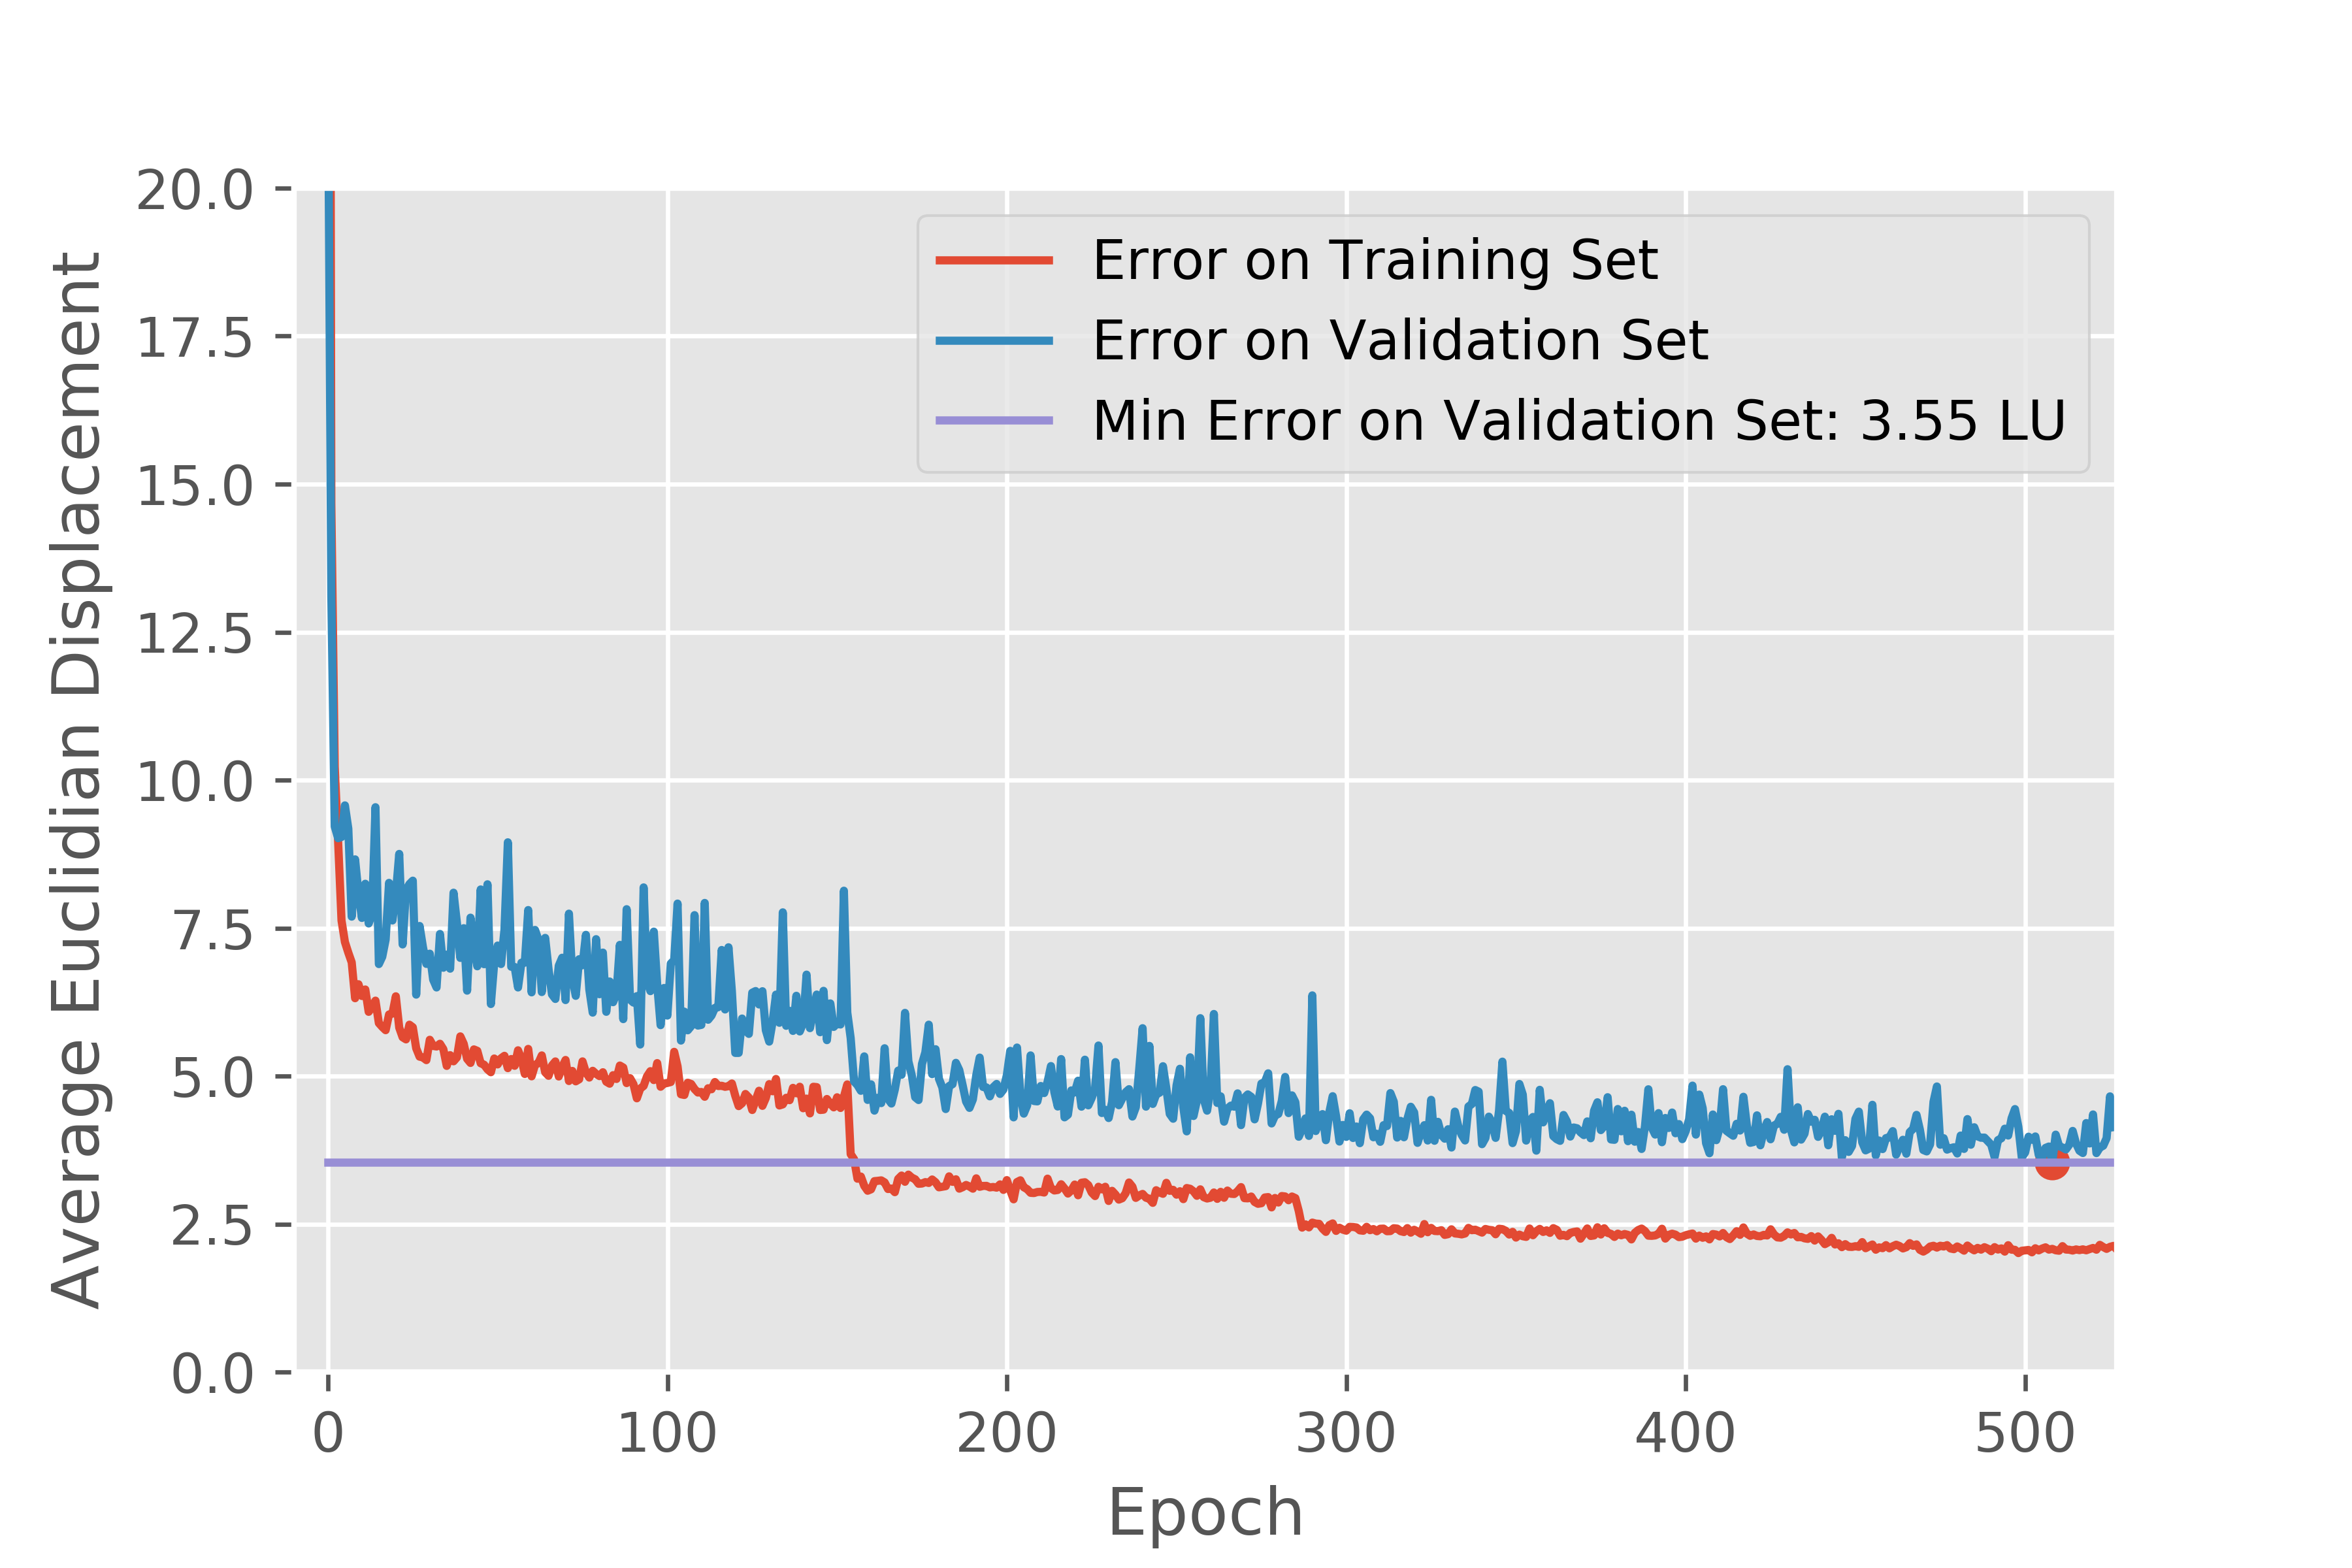
\includegraphics[width=0.99\textwidth]{figures/reg_plot1.pdf}
	\caption{Development of the average euclidean displacement by epoch on the training- and validation set.}
	\fontsize{3}{2}
	\label{fig:autoencoder_architecture}
\end{figure}

\subsubsection{Limitations of the Model}
This experiment is an attempt to show the principle ability to use convolutional neural network to solve a task with a time-series as input. This special posed task of the inverse problem of ECG gave comparably good results. This shows that the neural network is able to process through a temporally random selected section of fixed length, which makes it clear that it recognizes a pattern in the signals regardless of the phase of the concentric wave.
The simulated heart contains of around 10000 elements on the surface, which can represent an approximate source of the concentric wave. While having 1024 simulation, having unique starting conditions, around 10\% of the available sources are already covered. 
The properties of a simulation differ only in the location of the pacing events that cause the concentric wave. It is possible that some training and test simulations differ very little from each other, if the locations of the pacing events are very close to each other. In this case it may not be possible to speak of a truly unknown data set. The average minimal distance from a test-simulation to the next training-simulation is around 2.47 LU. It shows that the neural network is trained with pacing positions, which are not far distant from the test-simulations. Furthermore, the neural networks average displacement of the predictions on the test-dataset is bigger than the average distance to the next training simulation.
Nevertheless, the same CNN is able to handle a dataset with additional Gaussian noise. The training on the same dataset with this noise with $\sigma=0.05$ got displacements as shown in table \ref{tab:noise}:

\begin{table}[h]
    \centering
    \begin{tabular}{|c|c|}
    \hline
    training set & test set\\
    \hline
    1.69 & 3.15 \\
    \hline
    \end{tabular}
    \caption{Average displacement of the prediction from the CNN on the training- and test-dataset, additional Gaussian noise with $\sigma=0.05$ is added to the normalized data (this means that a 5\% error is included).}
    \label{tab:noise}
\end{table}

The average displacement on the test-dataset did not increase much (a difference of 0.04LU).
% Next:
    % more noise, geometrical noise
    % more complex simulations
    %

